\documentclass[a4paper, titlepage, abstract = true]{scrreprt}
\usepackage{lmodern}
\usepackage[T1]{fontenc} % font encoding
\usepackage[version=4]{mhchem} % chemical formula
\usepackage{siunitx} % e.g. \SI{1}{cm}  
\usepackage{graphicx} % figure
\graphicspath{{./fig/import/}} % path of figure
\usepackage{amsmath, amssymb} % for math
\usepackage{bxtexlogo} % logo such as "\pdftex"
\bxtexlogoimport{*,**} % setting for bxtexlogo
\usepackage[example]{cnltx} % for TeX/LaTeX command

\usepackage[hidelinks, draft = false, pdfusetitle]{hyperref} % hyperlink

\hypersetup{% setting hyperref
  bookmarksnumbered=true,
  bookmarksopen=true,
  bookmarkstype=toc,
  pdfborder={0 0 0},
  colorlinks = false
}

\usepackage{footnotebackref}
\usepackage{cleveref} % cross reference
% \crefname{type}{singlur form}{plural form}
\crefname{equation}{eq.}{eqs.}
\crefname{table}{table}{table}
\crefname{figure}{figure}{figures}
\crefname{chapter}{chapter}{chapters}
\crefname{section}{section}{sections}
\usepackage{booktabs}
\usepackage{sty/titlelayout} % fix \maketitle
\subject{Master thesis}
\title{A {\LaTeX} Template for Theses}
\author{Takumi Noguchi}
\affiliation{Department of Engineering 
Graduate School of Engineering, \\ 
Kochi University of Technology, Kohno Lab. Kami, Kochi, Japan}
\date{\today}

\usepackage{xparse}
\NewDocumentCommand\etc{}{\textit{etc.}}

\usepackage[%
backend = biber,%
articletitle = false,%
url = false,%
doi = false,%
eprint = false,%
isbn = false,%
sortcites = true, % \cite{paper1, paper2, paper3} -> [1-3]
style = phys%
]{biblatex} % use "biblatex"
\addbibresource{reference/reference.bib}
%
\DeclareFieldFormat[article]{journaltitle}{\mkbibemph{#1}}
%
% replace journal name with its abbreviations
%
\DeclareSourcemap{
    \maps[datatype=bibtex, overwrite=true]{
        \map{
            \step[fieldsource=Journal,
                match=\regexp{Applied\sPhysics\sLetters},
                replace={Appl. Phys. Lett.}]
            \step[fieldsource=journal,
                match=\regexp{Journal\sof\sNanoscience\sand\sNanotechnology},
                replace={J. Nanosci. Nanotechnol.}]
            \step[fieldsource=journal,
                match=\regexp{Japanese\sJournal\sof\sApplied\sPhysics},
                replace={Jpn. J. Appl. Phys.}]
        }
    }
}

\begin{document}

\maketitle

\tableofcontents

\begin{abstract}
    This study is very excellent.
\end{abstract}

\chapter{序論} \label{chap:introduction}

\section{研究背景と目的} \label{sec:chap::introduction_background}

{\TeX}/{\LaTeX}はレポートや学位論文などのような文書を作成する際に広く使われている.
これは,{\TeX}/{\LaTeX}がマークアップ方式で文書を作成するため,
ユーザーは文書の論理構造と体裁を容易に分離できるからである.
学生が文書の論理構造のみに注力するため,多くの研究室で{\LaTeX}テンプレートが配布されている.

ところが,研究者は必ずしも{\LaTeX}に詳しいというわけではないため,
そのテンプレートは古く,現代のモダンな{\TeX}システムにそぐわない場合も少なくない.
このことが原因で,モダンな{\TeX}システムでこれらのテンプレートを使うと
文書の体裁がひどくなったりエラーが発生したりといったことが起こることがある.

このテンプレートは,モダンな{\LaTeX}環境で使える
{\LuaLaTeX}を用いた学位論文のテンプレートを提供する.

\section{特徴} \label{sec:chap::introduction_feature}

このテンプレートでは
\begin{itemize}
    \item ドキュメントクラスとして\cls*{ltjsreport}を,
    \item ビルドツールとして\verbcode{llmk}を
\end{itemize}
採用している.

\section{数式と相互参照} \label{sec:chap::introduction_equation}

\emph{インライン}数式は,\verbcode{$ formula $}の形で入力する.
例えば,$x + y$や$a = b$である.

一行からなる\emph{ディスプレイ}数式の場合には,
\verbcode{\[}と\verbcode{\]}で囲むか\env*{equation}環境を用いる.
例えば,\verbcode{\[}と\verbcode{\]}で囲んだ場合,
\[
    y = ax^2 + bx + c
\]
のようになり,\env*{equation}環境%
\footnote{%
    \env*{equation*}環境を用いた場合,式番号はつかない.
    一般に,数式を入力する環境でスター付きのものを用いた場合,
    その数式に番号がつかなくなる.
}%
を用いた場合には
\begin{equation}
    y = \sin x + 2 (x + y) + \sqrt{x} + \sqrt[3]{x} \text{.}
    \label{eq:chap::introduction_sec::background_sinparensqrt}
\end{equation}
のようになる.
下の数式には番号がついており,\cs*{label}コマンドでラベルづけすることができる.
そして,\ref{eq:chap::introduction_sec::background_sinparensqrt}
のように,\cs*{ref}コマンドでその式を参照できる.
\cs*{ref}コマンドで参照できるのは式だけではない.
章や節,図や表なども参照できる.
数式の場合には,
\eqref{eq:chap::introduction_sec::background_sinparensqrt}
のように\cs*{eqref}コマンドも使えるが,
\cs*{cleveref}パッケージが提供する
\cs*{cref}や\cs*{Cref}コマンドを用いることを推奨する.
なお,\cs*{Cref}コマンドは文頭用である.

複数行からなるディスプレイ数式を入力する場合には,
\pkg*{amsmath}パッケージが提供する数式環境で適切なものを選ぶ必要がある.
通常は\env*{align*}環境を用いればよい.例えば
\begin{align}
    \sin^2 x + \cos^2 x = 1,
    \label{eq:chap::introduction_sec::equation_sincos} \\
    \tan x = \frac{\sin x}{\cos x}
    \label{eq:chap::introduction_sec::equation_tan}
\end{align}
である.
「\verbcode{&}」を\env*{align}環境中に置くことで,
それらの式を整列することができる:
\begin{align*}
    \cos 2x & = \cos^2 x - \sin^2 x      \\
            & = 1 - 2 \sin^2 x           \\
            & = 2 \cos^2 x - 1 \text{.}
\end{align*}

\section{表と図} \label{sec:chap::introduction_table}

表を入力するには以下のようにする:
\begin{table}[htbp]
    \centering
    \caption{\ce{SiC}ナノワイヤの製法}
    \label{tab:chap::introduction_sec::introduction_sicnanowire}
    \begin{tabular}{ccc}
        \toprule
        原料       & 基板    & 触媒    \\ \midrule
        サッカリン & \ce{Si} & \ce{Fe} \\
        サッカリン & \ce{Si} & \ce{Ni} \\
        \bottomrule
    \end{tabular}
\end{table}

図を取り込むには,以下のようにする:
\begin{figure}[htbp]
    \centering
    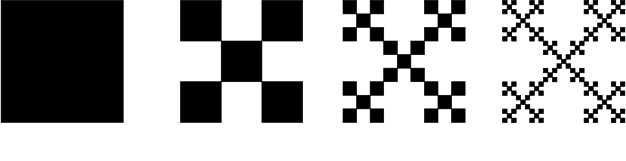
\includegraphics[width=100mm]{vicsek.pdf}
    \caption{ヴィチェック雪片の1,2,3段階目}
    \label{fig:chap::introduction_sec::introduction_vicseksnowflake}
\end{figure}

\cref{tab:chap::introduction_sec::introduction_sicnanowire}
や\cref{fig:chap::introduction_sec::introduction_vicseksnowflake}.
とすることで,表や図も\cs*{cref}コマンドで参照できる.

\section{文献の参照} \label{sec:chap::introduction_citation}

\cite{10.1093/jmicro/dfaa015}のように
\cs*{cite}コマンドで他の文献を参照できる.
\cite{10.1093/jmicro/dfaa015,Hayashi:2020:1533-4880:3038,Ishida_2019,doi:10.1063/1.4894003}
のように,複数の文献を一度に参照することもできる.
文献参照のためには,\verbcode{.bib}ファイルに文献のデータを記録する必要があり,
そのデータは\pkg*{biblatex}パッケージが提供する
\cs*{addbibresource}コマンドで取り込む.
このテンプレートでは,「\verbcode{phys}」という参照スタイルを採用している.

なお,\pkg*{biblatex}パッケージを用いる場合,文書を以下のようにしてビルドする:
\begin{itemize}
    \item ターミナル上で「\verbcode{lualatex thesis}」を実行する,
    \item ターミナル上で「\verbcode{biber thesis}」を実行する,
    \item ターミナル上で「\verbcode{lualatex thesis}」を実行する.
\end{itemize}

\section{ビルドの自動化} \label{sec:chap::introduction_autobuild}

上記のような手順は\verbcode{llmk}というツールを用いることで自動化できる.
\verbcode{llmk}を利用するためには,
Github上の\verbcode{llmk}のページ%
\footnote{\url{https://github.com/wtsnjp/llmk}}%
から
クローンする必要がある.

\printbibliography[title=Reference, heading=bibintoc]
\end{document}
